\chapter{Experimental Evaluation}
\label{chap:evaluation}

This chapter instantiates the framework defined in
Chapter~\ref{chap:construction} on a corpus of Type 1 and Type 2 diabetes guidelines.
Chapter~\ref{chap:construction} defined a four-stage architecture together with
the schema, extraction rules, and normalisation procedures configured for the
diabetes guideline corpus;
this chapter is the diabetes-specific instantiation and owns all concrete
details: corpus composition, tool choices, implementation decisions,
quantitative outcomes, and an analysis of where the pipeline succeeded and
where it did not. The sections follow the pipeline stages: corpus
selection~(Section~\ref{sec:exp_data}), document ingestion and
preprocessing~(Section~\ref{sec:exp_ingestion}), knowledge graph
construction~(Section~\ref{sec:exp_norm}), question
generation~(Section~\ref{sec:exp_questions}), evaluation of the question
catalogue~(Section~\ref{sec:exp_quality}), and
limitations~(Section~\ref{sec:exp_limitations}).

\section{Data Sources and Corpus}
\label{sec:exp_data}

The corpus is drawn from four guideline-producing organisations: the
American Diabetes Association~(ADA)\footnote{https://www.diabetes.org/}, the National Institute for Health and
Care Excellence~(NICE)\footnote{https://www.nice.org.uk/}, the International Diabetes Federation~(IDF)\footnote{https://www.idf.org/}, and
Diabetes Canada\footnote{https://www.diabetes.ca/}. Together they satisfy the four selection criteria defined
in Section~\ref{sec:corpus}. The corpus comprises eight documents, each
processed as one ingestion unit. Table~\ref{tab:corpus} reports the
structural properties measured at the output of the ingestion stage.
The IDF document served as the initial development document for the
extraction pipeline before the implementation was extended to the other
three guideline families.

\begin{table}[!ht]
\centering
\small\setlength{\tabcolsep}{5pt}
\begin{tabular}{p{2.1cm} p{5.2cm} r r r r p{2.0cm}}
\hline
\textbf{Organisation} & \textbf{Document} & \textbf{Year} & \textbf{Pp.}
                      & \textbf{Rec.} & \textbf{Tab.} & \textbf{Units} \\
\hline
ADA
  & Standards of Care in Diabetes
  & 2026 & 377 & 176 & 113 & mg/dL \\[2pt]
NICE
  & NG17: Type~1 Diabetes in Adults
  & 2026 &  64 & 100 &   0 & mmol/L, \newline mmol/mol \\[2pt]
NICE
  & NG28: Type~2 Diabetes in Adults
  & 2026 & 124 & 116 &   0 & mmol/L, \newline mmol/mol \\[2pt]
IDF
  & Global Clinical Practice Recommendations
  & 2025 & 112 &   10 &  21 & mmol/L \\[2pt]
Diabetes Canada
  & CPG 2018, Chapter~3
  & 2018 &   6 &  2 &  5 & mmol/L \\[2pt]
Diabetes Canada
  & CPG 2018, Chapter~4
  & 2018 &   4 &  2 &   1 & mmol/L \\[2pt]
Diabetes Canada
  & CPG 2018, Chapter~8
  & 2018 &   5 &  5 &  1 & mmol/L \\[2pt]
Diabetes Canada
  & CPG 2018, Chapter~9
  & 2018 &   7 &  8 &   1 & mmol/L \\[2pt]
\hline
\textbf{Total}
  & \textit{8 documents, 4 organisations}
  & & \textbf{699} & \textbf{419} & \textbf{142} & \\
\hline
\end{tabular}
\caption{Corpus documents and structural properties.}
\label{tab:corpus}
\end{table}

\subsection{Corpus against Selection Criteria}
\label{sec:corpus-criteria}

\paragraph{Geographic and systemic diversity.}
The four organisations publish from different national and international
contexts: the ADA in the United States, NICE in England and Wales, Diabetes
Canada in Canada, and the IDF as an international federation. Selecting
organisations from more than one context gives variation in guideline origin,
publishing convention, and recommendation structure, rather than restricting
the corpus to a single publisher.

\paragraph{Clinical coverage.}
Across the eight documents the corpus addresses all five clinical domains
identified in Section~\ref{sec:corpus}: diagnosis and classification~(ADA
Table~2.1, Canada Ch.~3), screening~(NICE NG17 Section~1.1, Canada Ch.~3),
glycaemic targets~(all four organisations), pharmacological management~(ADA
Section~9, NICE NG28, IDF, Canada Ch.~8--9), and monitoring~(NICE NG17
Section~1.5, Canada Ch.~4). No domain is covered by a single organisation only.

\paragraph{Format diversity.}
NICE documents present recommendations as numbered statements, and convey
their strength through wording rather than a grade label. In the versions
processed here, the NICE guidelines contained [N] embedded tables. The ADA
document combines numbered recommendations, each with an evidence grade, with
113 embedded tables in a three-column page layout. The IDF uses prose and two-column
care-tier tables with no structured recommendation numbering. The Canada
chapters are journal articles with graded recommendations embedded in
continuous clinical commentary.

\paragraph{Recommendation specificity.}
All documents contain actionable recommendations specifying drug choices,
numerical targets, or monitoring schedules. High-level policy documents were
excluded because they do not produce meaningful pharmacological or measurement
entities in the schema.

\subsection{Structural Heterogeneity in Practice}
\label{sec:heterogeneity-practice}

NICE contributes 496 chunks, 216 structured recommendations across its two documents and
zero tables; the ADA contributes 1,832 prose chunks, 176 structured
recommendation elements, and 113 reconstructed tables; the IDF
contributes 10 recommendation elements and 21 tables; the Canada chapters
contributes 107 chunks, 8 tables and 17 recommendations. The measurement unit column illustrates the
unit inconsistency: the ADA uses mg/dL for plasma glucose while the other
three use mmol/L, and NICE reports HbA1c in mmol/mol rather than as a
percentage. These three dimensions of heterogeneity directly shaped every
design decision in the ingestion and extraction stages.

Figure~\ref{fig:corpus} shows the number of chunks, recommendations, tables,
and sections extracted per organisation, visualising the same structural
volume reported in Table~\ref{tab:ingestion} and highlighting NICE's absence
of tables and the ADA's dominance in chunk and table count..

\begin{figure}[!ht]
    \centering
    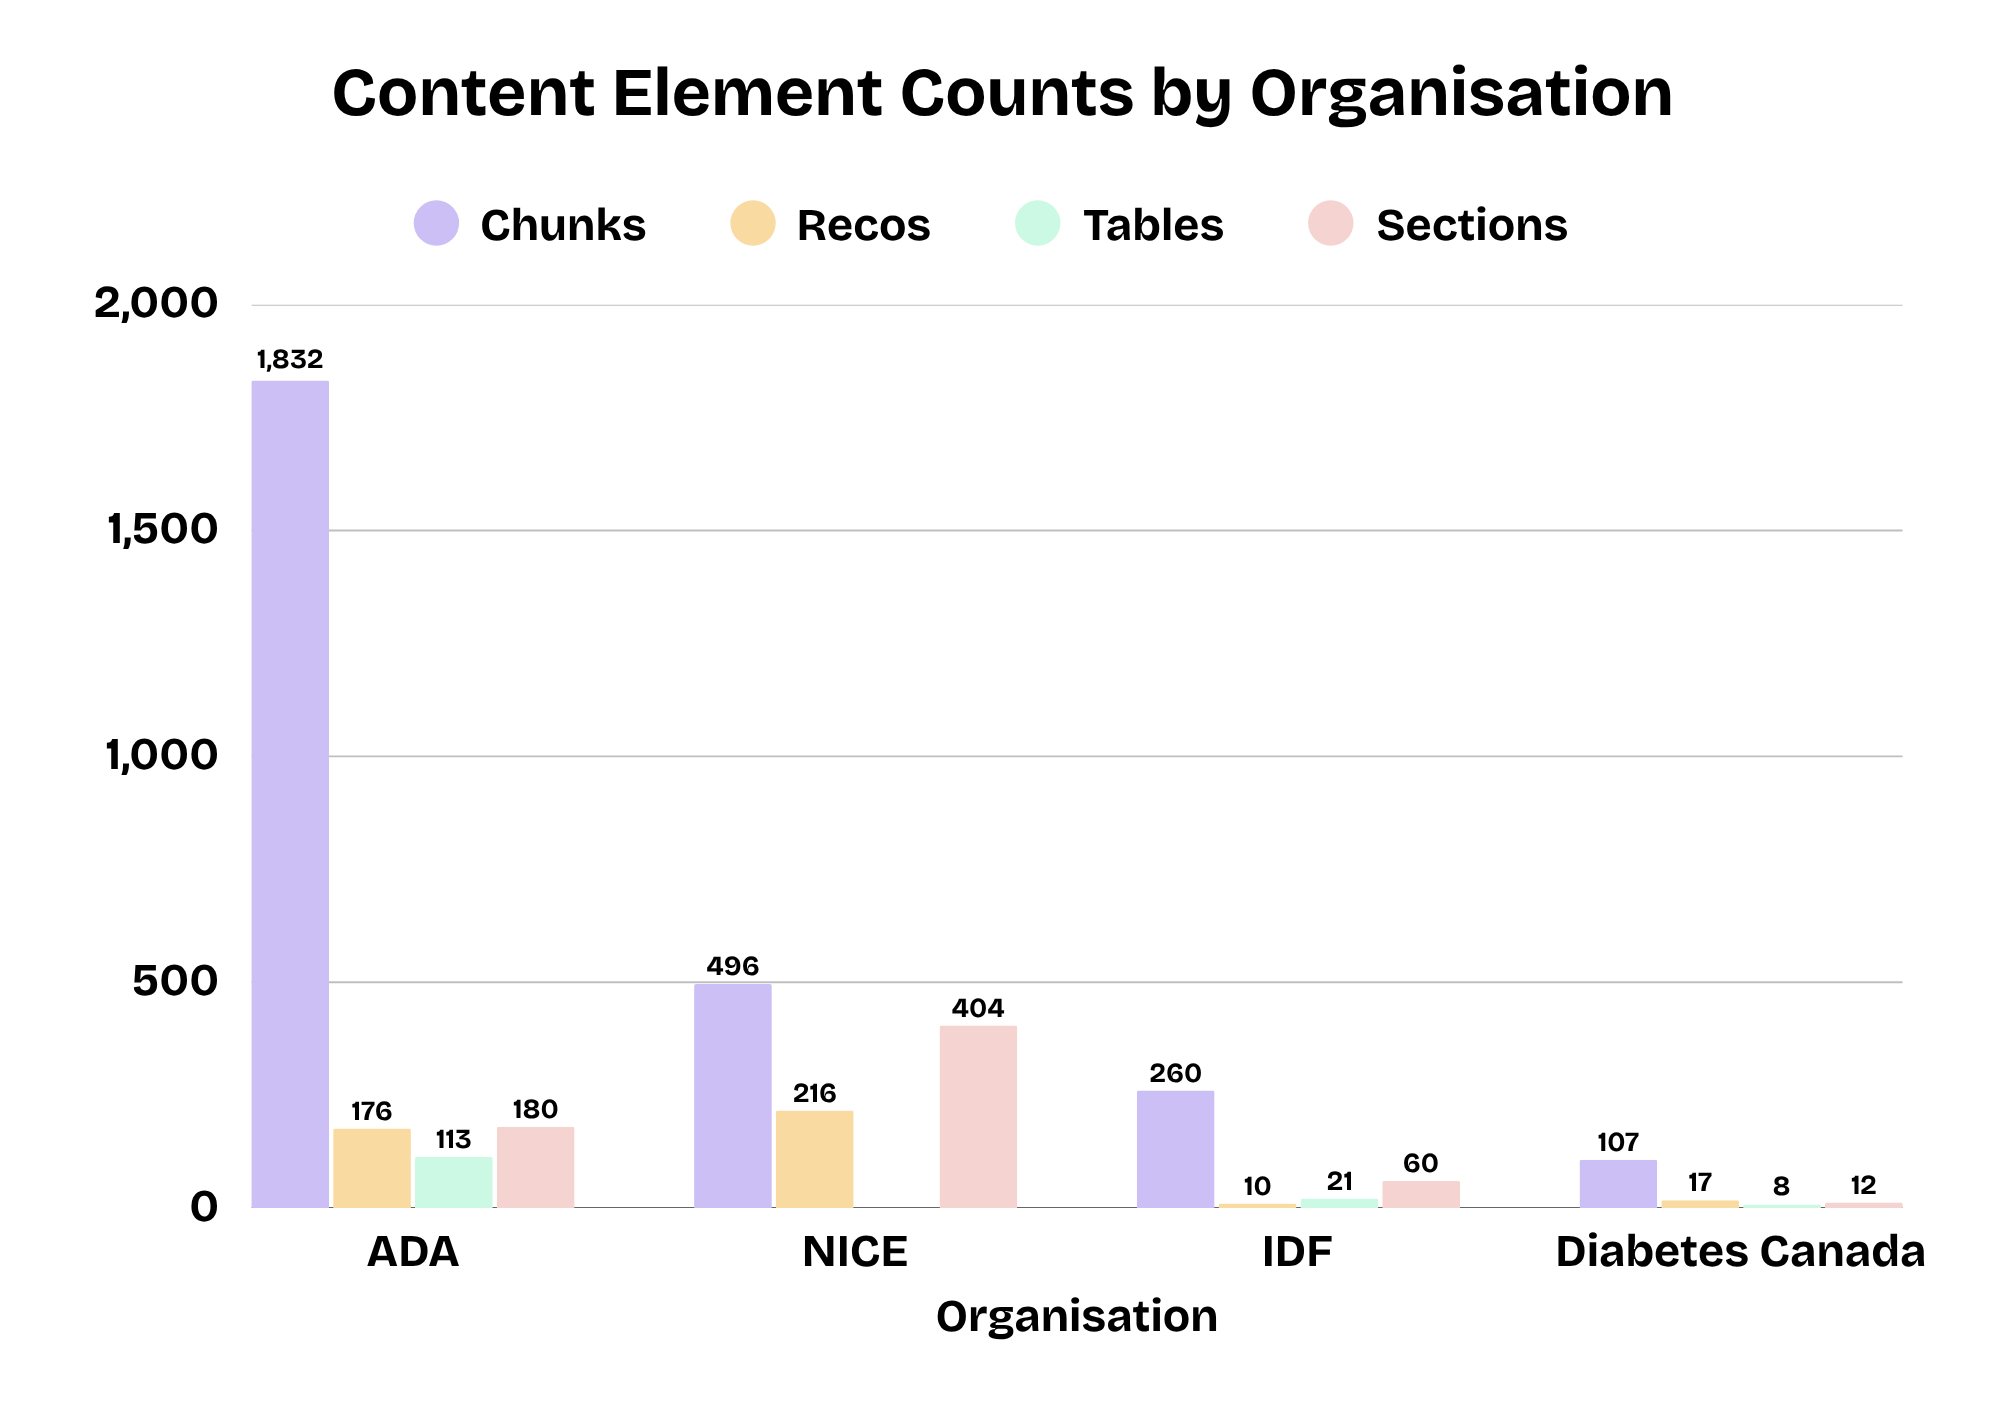
\includegraphics[width=\textwidth]{inc/figures/corpus.png}
    \caption{Structural profile of the guideline corpus by organisation.}
    \label{fig:corpus}
\end{figure}

\section{Document Ingestion and Preprocessing}
\label{sec:exp_ingestion}

The ingestion stage applies $\varphi: \mathcal{D} \rightarrow 2^{\mathcal{E}}$
to each of the eight corpus documents. This section describes the parsing
tool, the document-family-specific text repairs required before extraction
could begin, and the resulting element counts.

\subsection{Document Parsing Tool}
\label{sec:exp_parsing}

The ingestion pipeline uses PyMuPDF~\cite{pymupdf2026}\footnote{PyMuPDF,
version 1.28.0, \url{https://pymupdf.readthedocs.io}.} (via the
\texttt{fitz} interface) as its primary PDF extraction engine and
\texttt{pdfplumber}~\cite{yang2025}\footnote{pdfplumber, version 0.11.10,
\url{https://github.com/jsvine/pdfplumber}.} for table extraction.
Docling~\cite{auer2024}\footnote{Docling, version 2.130.0,
\url{https://github.com/docling-project/docling}.} is retained in the ingestion
script as an optional conversion step, but it was not adopted. Its output is not
used by the downstream stages, and the element records are unchanged when it is
unavailable. On five pages of one Diabetes Canada chapter, block extraction with
PyMuPDF took 0.03 seconds and table extraction with pdfplumber 0.89 seconds (mean
of five runs), against 114 seconds for a Docling conversion of the same pages on
the development laptop (CPU only),\footnote{CPU 1.70 GHz, 12 cores; RAM 16GB; Intel UHD Graphics.} The text export
requested by the script also carries no page numbers or coordinates. Every element
record needs a page range, and reading order and heading recovery need block
coordinates, so the element records are built from PyMuPDF blocks and pdfplumber
tables. No systematic comparison of the parsers was carried out.

PDF extraction from scientific documents introduces known artefacts,
including ligature encoding, token-boundary errors, and multi-column layout
bleed~\cite{bast2017}. PyMuPDF is the base of the pipeline because several
corpus-specific steps need direct access to raw text blocks with page
identifiers, font sizes, and bounding boxes. Reading order and heading
recovery use the block coordinates and font sizes, and the ADA and IDF
recommendation extractors work on the ordered raw blocks rather than on merged
section text. A repair for concatenated words, written for the Diabetes Canada
PDFs, is applied to every extracted block and to the table cells of
journal-style documents. Tables are reconstructed with \texttt{pdfplumber}.

The output for each document is a set of typed JSONL files:
\texttt{chunks.jsonl} for \textsc{Prose} elements,
\texttt{recommendations.jsonl} for \textsc{Recommendation} elements, a
\texttt{tables/} directory of CSV files for \textsc{Table} elements, and
\texttt{sections.jsonl} for \textsc{Section} elements. These constitute
the intermediate representation consumed by the extraction stage.

\subsection{Text Repair Passes}
\label{sec:exp_repair}

The ingestion implementation contains several document-family-specific
repairs and extraction rules that were added after inspecting failures in
the raw PDF output. Table~\ref{tab:repair} summarises the ones that directly
affected the corpus representation used here.

\begin{table}[!ht]
\centering
\small\setlength{\tabcolsep}{5pt}
\begin{tabular}{p{0.7cm} p{3.2cm} p{2.5cm} p{4.8cm}}
\hline
\textbf{Fix} & \textbf{Artefact} & \textbf{Affected families}
              & \textbf{Repair operation} \\
\hline
A & Word concatenation and camelCase runs
    (e.g.\ \texttt{Ageofonset}, \texttt{Type1diabetes})
  & Diabetes Canada
  & Split at digit--letter and camelCase boundaries when
    concatenation density exceeds a threshold \\[4pt]
B & Canada numbered recommendations parsed as prose
    (\texttt{"1. Diabetes should..."})
  & Diabetes Canada
  & Dedicated regex \texttt{CANADA\_RECO\_RE} promotes
    matched blocks to \textsc{Recommendation} elements \\[4pt]
C & ADA boxed recommendation text fused into single spans by PyMuPDF
  & ADA
  & Separate extractor \texttt{extract\_ada\_recommendation\_blocks}
    runs on raw blocks before section merge \\[4pt]
D & NICE table captions consumed as section headings
  & NICE
  & \texttt{looks\_like\_heading()} short-circuits on
    \texttt{NICE\_TABLEISH\_RE} matches when NICE numbering
    is active \\[4pt]
E & IDF ``Optimal / Basic / Recommended Care'' prose blocks
    not matched as recommendations
  & IDF
  & \texttt{extract\_idf\_recommendations()} with pattern
    \texttt{IDF\_CARE\_RE} promotes matching blocks \\[4pt]
F & Duplicate section headings or repeated heading blocks in the extracted page content
  & ADA, NICE, IDF
  & Per-page deduplication by title string in
    \texttt{recover\_headings()} \\[4pt]
\hline
\end{tabular}
\caption{Document-family-specific text repair passes.}
\label{tab:repair}
\end{table}

Fix~A is the most structurally significant for the Canada documents. The
\textit{Canadian Journal of Diabetes} typesetting pipeline produces PDF text
streams in which word boundaries are not encoded as whitespace: the string
\texttt{Ageofonset} must be reconstructed as \texttt{Age of onset} before
any pattern matching is possible. The repair applies unconditional digit--letter
splitting followed by conditional camelCase splitting when the density of
lowercase--uppercase transitions in a block exceeds 4\%.

Fix~C and Fix~D reflect the two most common extraction failures during
development: ADA clinical directives were being silently swallowed into
prose chunks, and NICE table captions were being misclassified as section
headings, producing spurious \textsc{Section} elements at the start of
tabular content.

No character- or token-level repairs were required for the IDF body text, whose Unicode streams are clean. Fix E instead addresses structural recognition of care-tier recommendation blocks.

\subsection{Ingestion Statistics}
\label{sec:exp_ingestion-stats}

Table~\ref{tab:ingestion} reports element counts after all repairs: the corpus
produces 2,695 chunks, 419 recommendation elements, and 142 tables, dominated by
the ADA document at 1,832 chunks and 176 recommendations, while the four Diabetes
Canada chapters, each covering only a few pages, contribute the fewest elements
individually. The 3,256 extracted content records represented by chunks,
recommendations, and tables form the principal inputs used by the downstream
extraction stages; the 656 section elements are consumed internally for
provenance annotation and are not passed forward.

\begin{table}[!ht]
\centering
\small
\begin{tabular}{llrrrr}
\hline
\textbf{Org.} & \textbf{Document} & \textbf{Chunks}
              & \textbf{Recos} & \textbf{Tables} & \textbf{Sections} \\
\hline
ADA          & Standards of Care 2026   & 1{,}832 & 176 & 113 & 180 \\
NICE         & NG17: Type~1 Diabetes    &   190   & 100 &   0 & 167 \\
NICE         & NG28: Type~2 Diabetes    &   306   & 116 &   0 & 237 \\
IDF          & Global CPR 2025          &   260   &   10 &  21 &  60 \\
Diab. Canada & CPG 2018 Ch.~3           &    30   &  2 &  5 &   3 \\
Diab. Canada & CPG 2018 Ch.~4           &    19   &  2 &   1 &   3 \\
Diab. Canada & CPG 2018 Ch.~8           &    23   &  5 &   1 &   3 \\
Diab. Canada & CPG 2018 Ch.~9           &    35   &  8 &   1 &   3 \\
\hline
\textbf{Total} &                        & 2{,}695 & 419 & 142 & 656 \\
\hline
\end{tabular}
\caption{Content-element counts after preprocessing.}
\label{tab:ingestion}
\end{table}

The ADA produces the largest chunk count (1,832) because its clinical directives are embedded in 377 pages of dense prose alongside structured recommendation elements. The Canada chapters produce relatively small chunk and recommendation sets because each chapter is short, but both prose chunks and explicitly extracted recommendation elements remain present in the intermediate representation. 
The IDF produces 10 recommendation elements through its dedicated care-level recommendation extractor, alongside 21 reconstructed tables.



\section{Knowledge Graph Construction}
\label{sec:exp_norm}

This section describes how the 3,256 content elements were converted into the
final Knowledge Graph $G$, covering entity and relation extraction, graph
database selection, entity deduplication, unit normalisation, cross-guideline
equivalence edges, and the resulting graph statistics.
\subsection{Entity and Relation Extraction}
\label{sec:extraction-impl}

Extraction is implemented as two scripts that follow the split defined in
Chapter~\ref{chap:construction}. Extraction-derived entities carry an \texttt{extract\_method} field where applicable.

\paragraph{Rule-based extraction.}
The rule extractor runs six passes in a fixed order. It first creates the
\textsc{Guideline} and \textsc{Organisation} nodes and the five canonical
\textsc{Condition} nodes. It then extracts \textsc{Recommendation} nodes from the
numbered recommendation records produced during ingestion, numerical targets from
chunk text, and table-derived nodes from the reconstructed tables. The last pass
creates the \textsc{equivalent\_to} relations once all documents have been
processed. The final graph contains 70 nodes labelled \texttt{rule}: 46
\textsc{GlycaemicTarget}, 14 \textsc{MonitoringProtocol} and 10
\textsc{TreatmentRecommendation}. A further 491 nodes are created by the same
script without a method label: 330 \textsc{Recommendation}, 139 \textsc{Table},
8 \textsc{Guideline}, 4 \textsc{Organisation}, and 5 each of \textsc{Condition}
and \textsc{Test}. A numerical target is linked to Type~1 or Type~2 diabetes only
when the surrounding text names exactly one of them.

\paragraph{Contextual extraction.}
The contextual extractor sends text chunks to a language model together with the
schema prompt shown in Appendix~\ref{app:extraction-prompts}. The reported graph
was produced with [[gpt-4o-mini through the OpenAI API]]\footnote{Model
identifier \texttt{gpt-4o-mini}, accessed through the OpenAI API,
\url{https://platform.openai.com/docs/models}.}, using
temperature~0 and a JSON response format. For each page, the prompt also contains
up to 20 facts already found by the rule extractor (numerical targets and short
recommendation summaries) as known context. The parser reads the JSON response but
does not check returned types against the schema. In the raw output, all 2,275
entities use declared types, but 2 of the 1,533 relations use undeclared types
(\textsc{researching} and \textsc{intervention}, one each); neither is part of the
final graph. Deduplication reduces the 2,275 entities to 1,942: \textsc{Drug} 627
to 438, \textsc{ClinicalCondition} 574 to 462 and \textsc{Intervention} 337 to 305,
while \textsc{Population} stays at 737. All 1,942 carry the same confidence value
of 0.7, so this field does not separate easy from hard extractions.


\subsection{Graph Database}
\label{sec:graph-db}

The Knowledge Graph is stored in Neo4j ~\cite{barrasa2023}\footnote{Neo4j [2026.04.0], \url{https://neo4j.com}.}
. Neo4j was chosen because it
stores both nodes and edges as first-class objects with arbitrary key-value
properties, which directly instantiates the property function
$\lambda: V \cup E \rightarrow 2^{\mathcal{P}}$. Provenance information such as the issuing organisation and source page
is stored directly on relations where it is available, without requiring
separate provenance nodes. Neo4j's Cypher query language also allows the
cross-guideline queries that motivate the graph to be expressed directly
as graph patterns. For example, the question \textit{which drugs are
recommended as first-line therapy by more than one organisation?} can be
answered by matching \textsc{first\_line\_for} relations and grouping the
results by organisation.

\subsection{Entity Deduplication}
\label{sec:dedup}

Deduplication applies the type-specific equivalence relation $\sim_\tau$
defined in Section~\ref{sec:normalisation} with two strategies.

For global node types (\textsc{Drug}, \textsc{Condition},
\textsc{ClinicalCondition}, \textsc{Intervention}, \textsc{Test}), two
records are equivalent when their normalised names satisfy
$\sigma(\text{name}_i) = \sigma(\text{name}_j)$, where $\sigma$ applies whitespace normalisation, lower-casing,
and type-specific synonym resolution. The implementation uses separate
alias mappings for tests, drugs, and clinical conditions. Representative entries are shown in Table~\ref{tab:synonyms}, which maps surface
forms such as \texttt{fpg} and \texttt{fasting plasma glucose} to the canonical
term \texttt{FPG}, and similarly collapses variant spellings of HbA1c and OGTT
into single canonical entities.

Deduplication of this kind is studied in the entity resolution
literature~\cite{getoor2012,christen2012}. Clinical concept
normalisation draws on the same principle as controlled vocabulary
resources such as the UMLS~\cite{bodenreider2004} and
RxNorm~\cite{hanna2013}, which map surface forms to canonical
identifiers; the synonym dictionary $\Delta$ plays an analogous
role within the scope of the corpus.

\begin{table}[!ht]
\centering
\small
\setlength{\tabcolsep}{6pt}

\begin{tabular}{p{0.68\textwidth} p{0.22\textwidth}}
\hline
\textbf{Surface form} & \textbf{Canonical form} \\
\hline

\texttt{fpg}, \texttt{fasting plasma glucose}, \texttt{fasting glucose}
&
\texttt{FPG}
\\[2pt]

\texttt{hba1c}, \texttt{a1c}, \texttt{glycated haemoglobin}
&
\texttt{HbA1c}
\\[2pt]

\texttt{ogtt}, \texttt{2h ogtt}, \texttt{2-h ogtt},
\texttt{75g ogtt}
&
\texttt{2h-OGTT}
\\

\hline
\end{tabular}
\caption{Selected synonym mappings for entity deduplication.}
\label{tab:synonyms}
\end{table}

Organisation-specific entities retain their source scope and use type-specific
identity keys rather than one common deduplication rule.
\textsc{GlycaemicTarget} records are keyed by metric, unit, comparison
operator, and value. \textsc{Recommendation} records use their recommendation
label and text, while \textsc{Table} and \textsc{MonitoringProtocol} records
use identifiers derived from the corresponding table or monitoring source. Records from different organisations are kept separate. For \textsc{GlycaemicTarget} records specifically, matching normalised thresholds across organisations are represented by an \textsc{equivalent\_to} edge as described below. 

\subsection{Unit Normalisation and Cross-Guideline Equivalence Edges}
\label{sec:unit-norm}

All plasma glucose threshold values are normalised to mmol/L using:

$$\text{value}_{\text{mmol/L}} = \frac{\text{value}_{\text{mg/dL}}}{18.0}$$

The divisor $18.0$ is the standard factor for converting plasma glucose
between mg/dL and mmol/L. The pipeline's corpus values confirm this:
the ADA states 126~mg/dL alongside $\geq 7.0$~mmol/L, and 200~mg/dL
alongside $\geq 11.1$~mmol/L,~\cite{ADA2026} both consistent with the divisor. The conversion is implemented in the shared helper
function \texttt{mgdl\_to\_mmolL}, imported by the rule extraction
script. HbA1c values are retained in their source unit, and the equivalent value on
the alternate scale is stored alongside it using the IFCC reference
relation~\cite{hoelzel2004}. Percentage values are converted to mmol/mol and mmol/mol values to
percentage, and the alternate representation is stored on the target node.
The current cross-guideline equivalence procedure, however, is restricted
to plasma-glucose targets represented in mmol/L.

\textsc{equivalent\_to} edges are created inside the rule extraction stage, after all documents
have been processed. The function \texttt{add\_cross\_guideline\_equivalences}
groups all \textsc{GlycaemicTarget} nodes by the tuple
$(\text{metric},\ \text{op},\ \text{round}(\text{value\_mmol\_L}, 1))$ and
adds directed \textsc{equivalent\_to} edges between matching target nodes
from different organisations within each group. The equivalence
check is exact equality on the rounded normalised value; no tolerance band
was applied. Although this operation is implemented in the rule-extraction
module, it runs only after the corpus-wide target extraction and numerical
normalisation pass; conceptually it therefore corresponds to the
normalisation stage defined in Chapter~\ref{chap:construction}.

Table~\ref{tab:equiv} lists the eight edges this process produced: three
organisations agree on an FPG threshold of 7.0 mmol/L, the same three agree
on a 2h-OGTT threshold of 11.1 mmol/L, and two further edges connect a Random
PG and a lower FPG bound between single pairs of organisations.

\begin{table}[!ht]
\centering
\small\setlength{\tabcolsep}{6pt}
\begin{tabular}{p{2.8cm} c p{2.4cm} p{2.4cm} p{2.4cm}}
\hline
\textbf{Metric} & \textbf{Op.} & \textbf{Value} & \textbf{Org. A}
                & \textbf{Org. B} \\
\hline
FPG          & $\geq$ & 7.0 mmol/L  & ADA            & Diabetes Canada \\
FPG          & $\geq$ & 7.0 mmol/L  & ADA            & IDF             \\
FPG          & $\geq$ & 7.0 mmol/L  & Diabetes Canada & IDF            \\
2h-OGTT      & $\geq$ & 11.1 mmol/L & ADA            & Diabetes Canada \\
2h-OGTT      & $\geq$ & 11.1 mmol/L & ADA            & IDF             \\
2h-OGTT      & $\geq$ & 11.1 mmol/L & Diabetes Canada & IDF            \\
Random PG    & $\geq$ & 11.1 mmol/L & ADA            & Diabetes Canada \\
FPG          & $<$    & 5.6 mmol/L  & ADA            & IDF             \\
\hline
\end{tabular}
\caption{Cross-guideline \texttt{equivalent\_to} edges after unit normalisation.}
\label{tab:equiv}
\end{table}

All eight edges concern diagnostic glucose thresholds, seven expressed as a
lower bound (\(\geq\)) and one as an upper bound for the normal range
(\(<5.6\)~mmol/L). The three FPG $\geq 7.0$~mmol/L edges form a triangle
across ADA, IDF, and Diabetes Canada; under the implemented equivalence
criterion their corresponding target nodes fall into the same normalised
group. No NICE plasma-glucose target nodes in the corpus satisfy the
implemented equivalence grouping.

Figure~\ref{fig:equiv} shows the eight edges as a matrix grouped by threshold,
making visible the two three-way agreements (FPG and 2h-OGTT) against the two
single-pair edges (Random PG and the normal-range FPG bound), and the absence
of NICE from every row.

\begin{figure}[!ht]
    \centering
    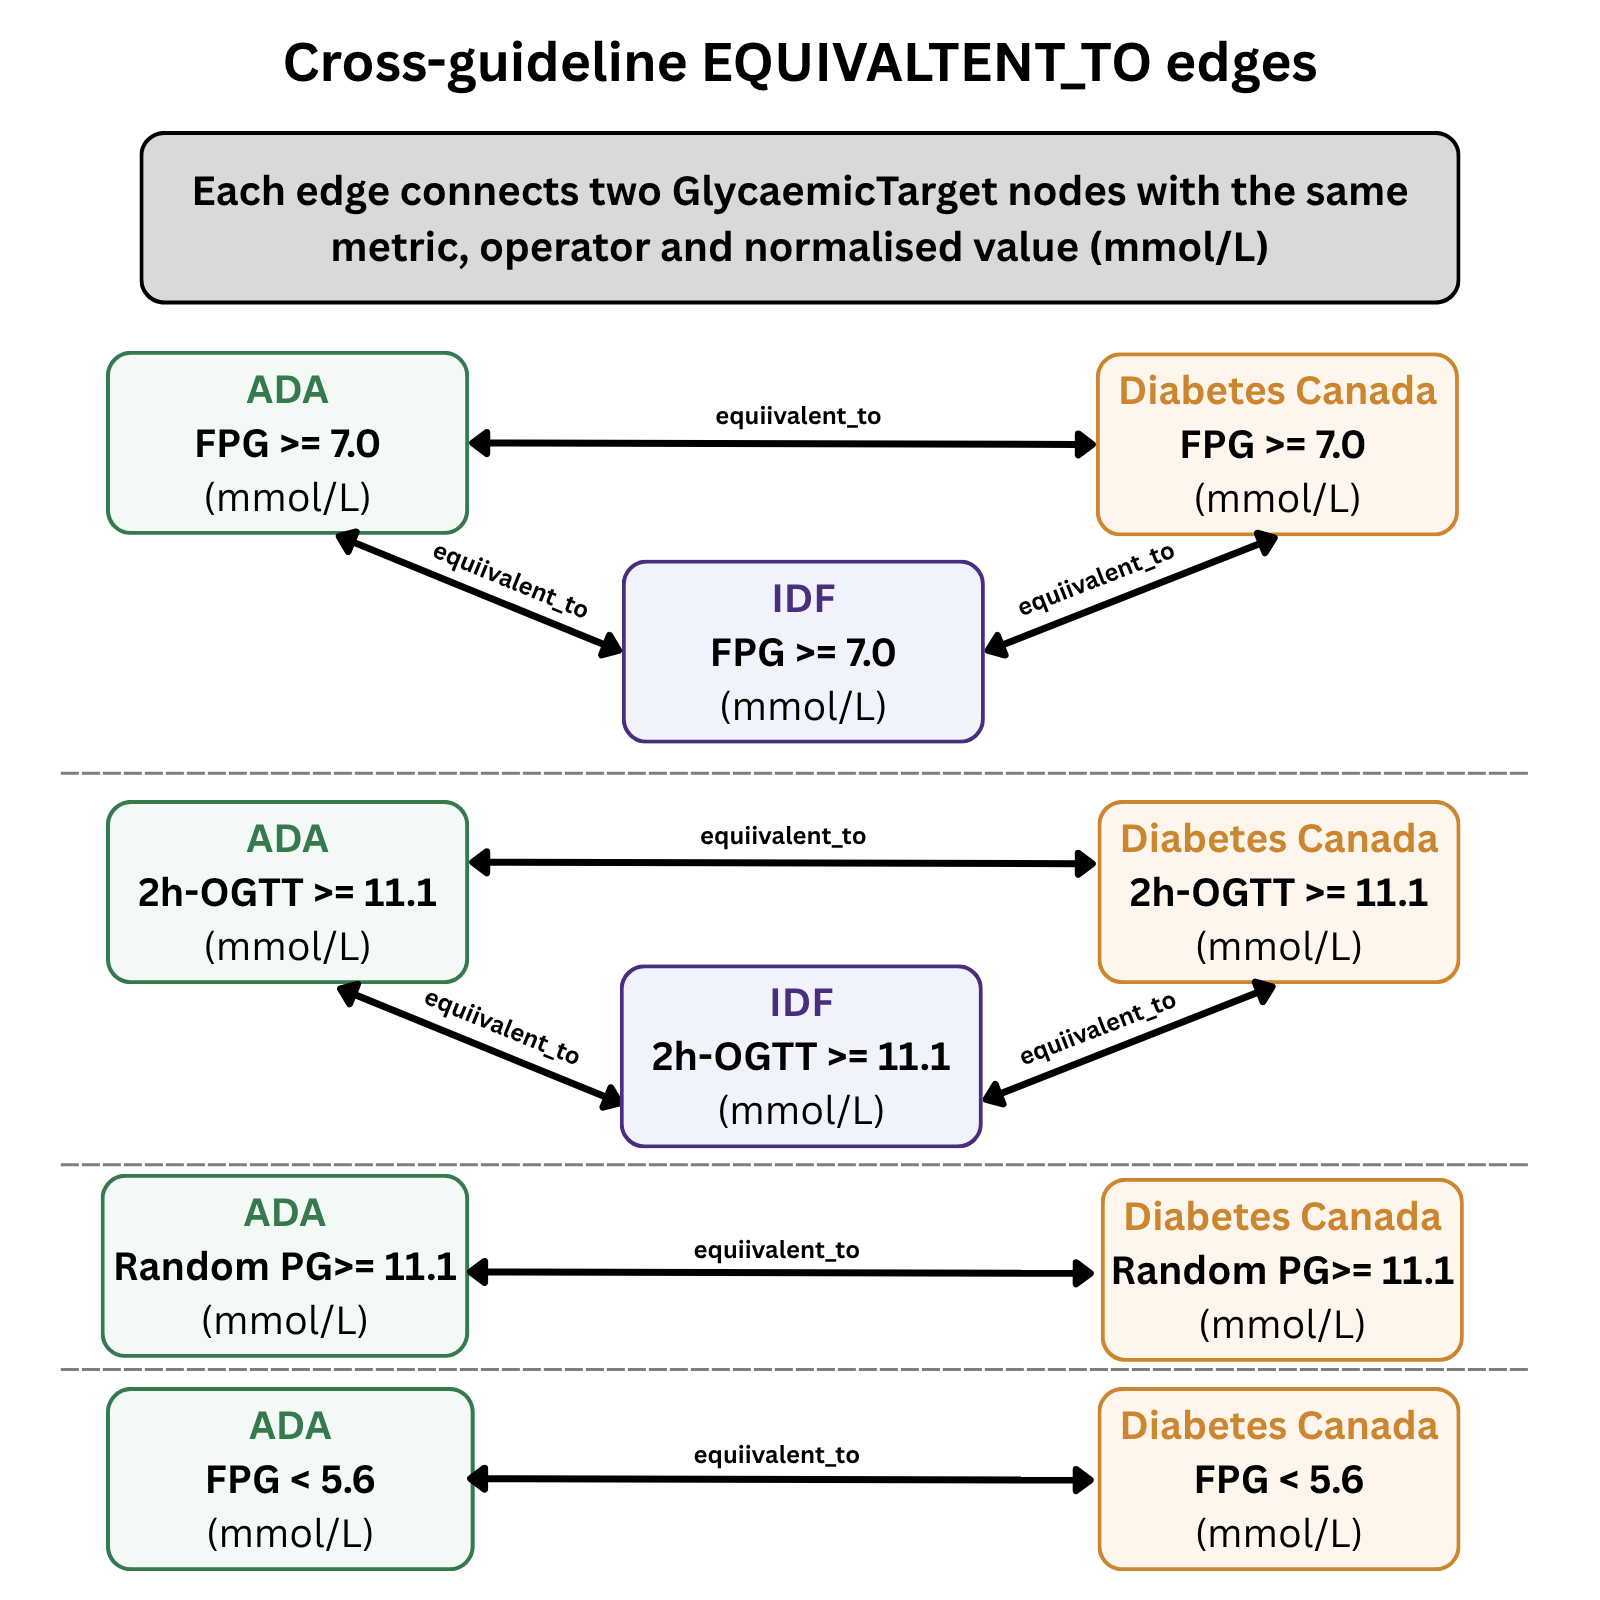
\includegraphics[width=0.85\textwidth]{inc/figures/equiv.png}
    \caption{Cross-guideline equivalence edges by diagnostic threshold.}
    \label{fig:equiv}
\end{figure}


\subsection{Final Graph Statistics}
\label{sec:graph-stats}

Tables~\ref{tab:nodes} and~\ref{tab:relations} report the composition of the
final Knowledge Graph after normalisation: 2,503 nodes across 13 types and 3,485
relations across 18 types, with \textsc{ClinicalCondition} and \textsc{Drug} the
largest node types and \textsc{mentioned\_in} the largest relation type at 1,409
edges. Figure~\ref{fig:graph-stats} shows how these node counts distribute across
the three scoping levels: global, organisation-scoped, and structural.


\begin{figure}[!ht]
    \centering
    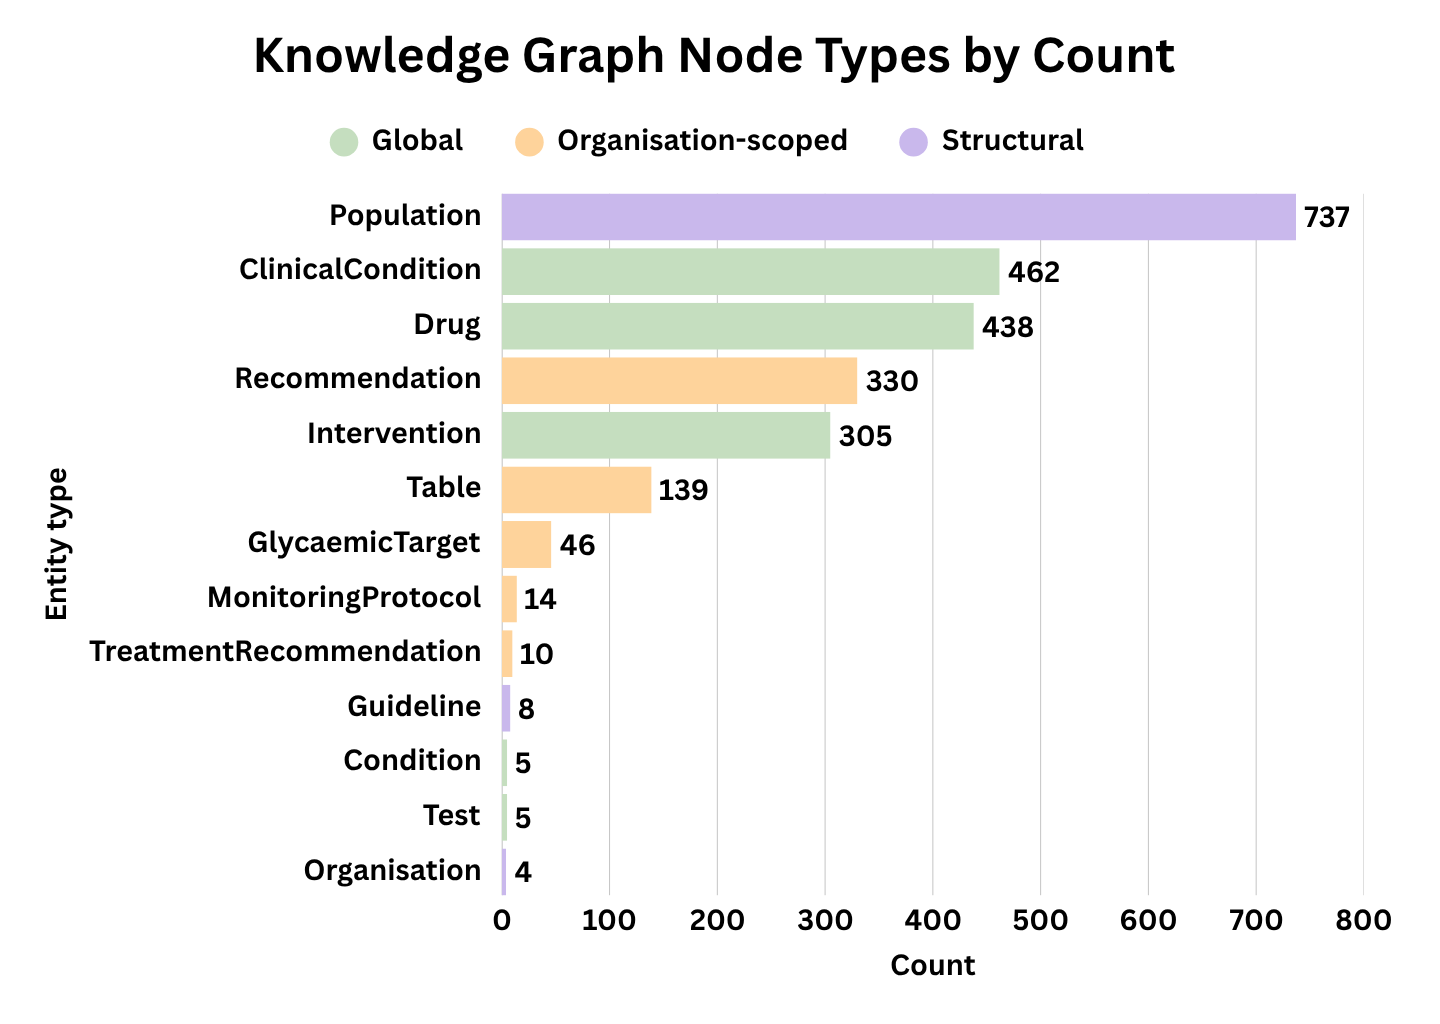
\includegraphics[width=\textwidth]{inc/figures/graph_stats.png}
    \caption{Node-type distribution by scoping level.}
    \label{fig:graph-stats}
\end{figure}

\begin{table}[!ht]
\centering
\small\setlength{\tabcolsep}{8pt}
\begin{tabular}{llr}
\hline
\textbf{Scoping level} & \textbf{Node type} & \textbf{Count} \\
\hline
Global
  & \textsc{Drug}                    & 438 \\
  & \textsc{ClinicalCondition}       & 462 \\
  & \textsc{Intervention}            & 305 \\
  & \textsc{Condition}               &   5 \\
  & \textsc{Test}                    &   5 \\
Organisation-scoped
  & \textsc{Recommendation}          & 330 \\
  & \textsc{Table}                   & 139 \\
  & \textsc{GlycaemicTarget}         &  46 \\
  & \textsc{MonitoringProtocol}      &  14 \\
  & \textsc{TreatmentRecommendation} &  10 \\
Structural
  & \textsc{Population}              & 737 \\
  & \textsc{Guideline}               &   8 \\
  & \textsc{Organisation}            &   4 \\
\hline
\textbf{Total}          &            & \textbf{2{,}503} \\
\hline
\end{tabular}
\caption{Final knowledge graph node counts.}
\label{tab:nodes}
\end{table}

\begin{table}[!ht]
\centering
\small\setlength{\tabcolsep}{8pt}
\begin{tabular}{llr}
\hline
\textbf{Semantic group} & \textbf{Relation type} & \textbf{Count} \\
\hline
Pharmacological
  & \textsc{recommended\_for}      & 551 \\
  & \textsc{manages}               & 272 \\
  & \textsc{first\_line\_for}      & 173 \\
  & \textsc{associated\_with}      & 157 \\
  & \textsc{contraindicated\_in}   & 110 \\
  & \textsc{second\_line\_for}     &  69 \\
  & \textsc{used\_with}            &  67 \\
Monitoring \& measurement
  & \textsc{requires\_monitoring}  &  53 \\
  & \textsc{measured\_by}          &  46 \\
  & \textsc{has\_target}           &  24 \\
  & \textsc{specifies\_target}     &  32 \\
  & \textsc{describes\_protocol}   &  23 \\
  & \textsc{has\_protocol}         &   4 \\
Cross-guideline \& provenance
  & \textsc{mentioned\_in}         & 1{,}409 \\
  & \textsc{has\_recommendation}   & 340 \\
  & \textsc{contains\_table}       & 139 \\
  & \textsc{publishes}             &   8 \\
  & \textsc{equivalent\_to}        &   8 \\
\hline
\textbf{Total}          &            & \textbf{3{,}485} \\
\hline
\end{tabular}
\caption{Final knowledge graph relation counts.}
\label{tab:relations}
\end{table}

\begin{figure}[!ht]
    \centering
    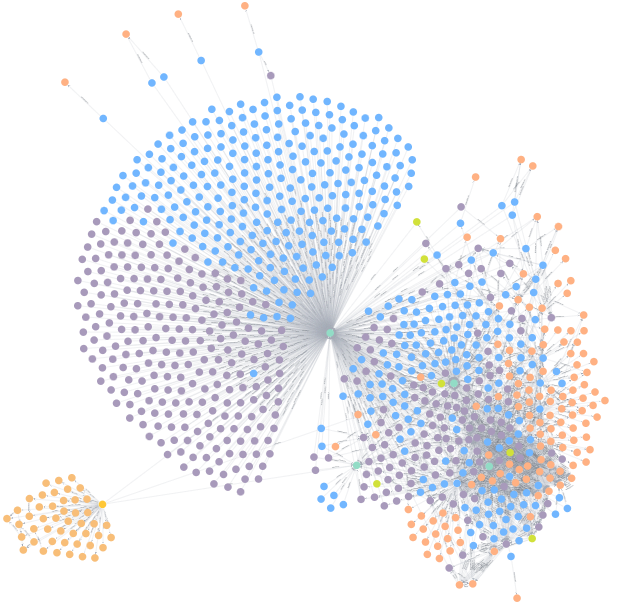
\includegraphics[width=\textwidth]{inc/figures/kg_full.png}
    \caption{Overview of the complete knowledge graph.}
    \label{fig:kg-full}
\end{figure}

The high \textsc{mentioned\_in} count (1,409, 40.4\%) reflects the provenance mechanism used to connect global entities to the guidelines in which they occur. These edges preserve cross-guideline occurrence information independently of more specific clinical relations. The next most frequent,
\textsc{recommended\_for}~(551), reflects the breadth of pharmacological
recommendations across the four families. The 438 \textsc{Drug} nodes and
462 \textsc{ClinicalCondition} nodes are high relative to the 5
\textsc{Condition} nodes. This reflects the schema design, in which a
small fixed set of canonical \textsc{Condition} nodes is pre-seeded,
while drug and clinical-condition mentions encountered during extraction may produce additional
nodes before synonym resolution.

\begin{figure}[!ht]
    \centering
    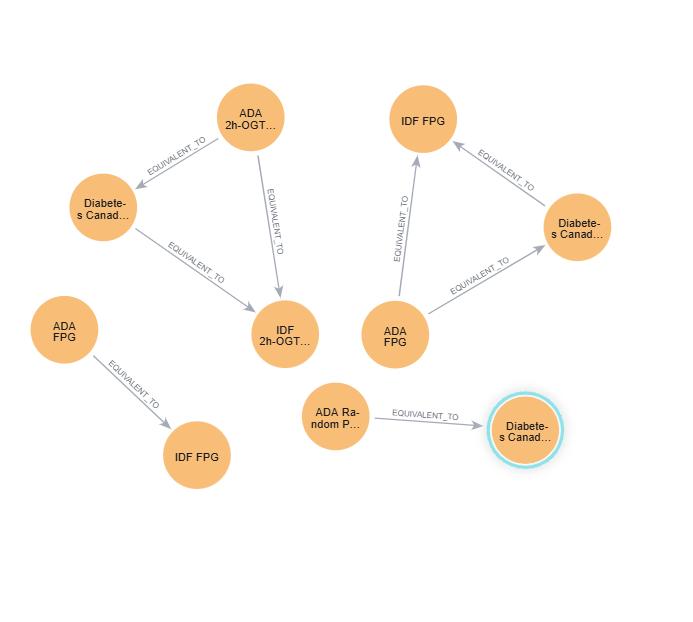
\includegraphics[width=\textwidth]{inc/figures/kg_equiv.png}
    \caption{Example of a cross-guideline equivalence relation in the knowledge graph.}
    \label{fig:kg-equiv}
\end{figure}

To illustrate the resulting graph structure at different levels of detail, Figure~\ref{fig:kg-equiv} shows an example of a cross-guideline equivalence relation. Figure~\ref{fig:kg-metformin} focuses on the neighbourhood of the drug metformin and illustrates how a single clinical entity can be connected to multiple relations and other entities. Finally, Figure~\ref{fig:kg-full} provides an overview of the complete knowledge graph.

\begin{figure}[!ht]
    \centering
    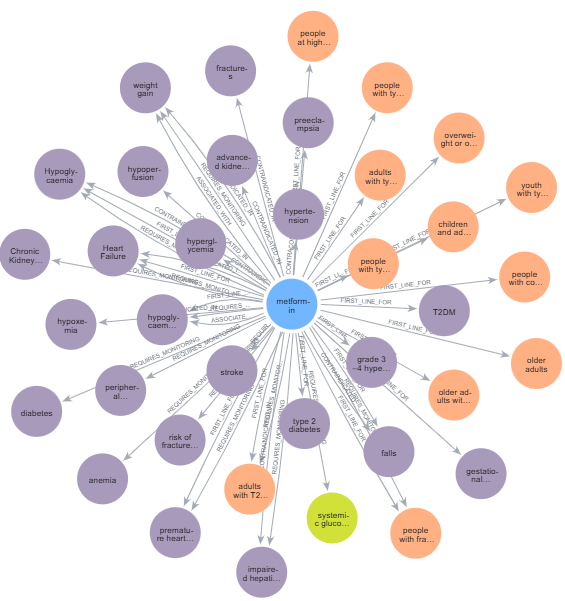
\includegraphics[width=\textwidth]{inc/figures/kg_metformin.png}
    \caption{Example of the graph neighbourhood of the drug metformin.}
    \label{fig:kg-metformin}
\end{figure}

\paragraph{Condition scoping of numerical targets.}
The extraction of a numerical target and its assignment to a diabetes
type are treated separately. A recognised numerical expression is maintained
as a \textsc{GlycaemicTarget} regardless of whether the surrounding text
identifies Type~1 or Type~2 diabetes. A disease-specific
\textsc{has\_target} relation is added only when the local context
identifies one of these types unambiguously.

This distinction was introduced after an implementation check showed that
the initial rule extractor used Type~2 Diabetes as the default condition
when no diabetes type could be determined from the local context. This
produced one \textsc{has\_target} relation for each of the 46 extracted
\textsc{GlycaemicTarget} nodes, even when the source text did not support
a Type~2-specific assignment. The condition-assignment rule was therefore
changed so that ambiguous targets remain in the graph without a
disease-specific relation.

With this correction, all 46 \textsc{GlycaemicTarget} nodes are retained,
while 24 \textsc{has\_target} relations are created. Seven originate from
the Type~1 Diabetes node and 17 from the Type~2 Diabetes node. Some targets
can be associated with both conditions when separate source contexts
support both assignments. The eight cross-guideline
\textsc{equivalent\_to} relations are unaffected because their construction
depends on the normalised target properties rather than on
\textsc{has\_target}.


\section{Question Generation}
\label{sec:exp_questions}

The question generation stage applies the three-function pipeline
$\gamma = \nu \circ \beta \circ \alpha$ defined in
Chapter~\ref{chap:construction} to the final Knowledge Graph,
where $\alpha$ is the graph-traversal targeting function,
$\beta$ is the language-model formulation function, and $\nu$ is
the rule-based validation function. In other words, a graph edge is
first selected as an anchor by $\alpha$, converted into question text
by $\beta$, and then checked against the same anchor by $\nu$.
This follows the schema-constrained prompting approach of
~\cite{caufield2024} and produces a validated catalogue
$\mathcal{Q}^+$.

Two question-generation runs are reported in this chapter and are analysed separately. The first run used Claude Opus 4.8 \footnote{Model identifier \texttt{claude-opus-4-8}, accessed through the Anthropic API, \url{https://docs.anthropic.com};}
 through the Anthropic API and was stopped before all eligible graph anchors had been processed because of practical token and cost constraints. This partial run produced a catalogue of 491 validated questions and was the source of the questions used in the human clinical review in Section~\ref{sec:exp_quality-human}. A subsequent run used gpt-4o-mini \footnote{Model identifier \texttt{gpt-4o-mini}, accessed through the OpenAI API, \url{https://platform.openai.com/docs/models}.}, using
the same final Knowledge Graph and provides the catalogue-level generation and validator statistics reported in this section. Results from the two runs are not pooled.

\subsection{Catalogue Overview}
\label{sec:q-overview}

In the GPT-4o-mini run, the targeting and generation pipeline produced 1,289 question records from eligible graph anchors. The rule-based validator accepted 1,280 questions (99.3\%) into \(\mathcal{Q}^+\) and routed 9 questions (0.7\%) to the flagged catalogue \(\mathcal{Q}^-\). No LLM fallback was required during this run. Of the 1,289 generated questions, 296 (23.0\%) were successfully produced with multiple-choice options, using LLM-generated distractors and a graph-locked correct answer. Of these, 294 were retained in the accepted catalogue after validation.


\subsection{Distribution by Relation Type}
\label{sec:q-by-relation}

Relation-type-driven question generation is an established approach in
knowledge-graph question generation. The distribution
reflects both the graph edge frequency and the per-type
sampling limits in $\alpha$.
Table~\ref{tab:q-relation} shows the question counts per relation type:
\textsc{recommended\_for} produces the most questions at 383, followed by
\textsc{manages} at 265, while \textsc{equivalent\_to}, despite drawing on only
eight graph edges, still produces 8 cross-guideline questions that no
single-guideline source could support.

\begin{table}[!ht]
\centering
\small\setlength{\tabcolsep}{8pt}
\begin{tabular}{p{4.2cm} r p{3.8cm}}
\hline
\textbf{Relation type} & \textbf{Questions} & \textbf{Question form} \\
\hline
\textsc{recommended\_for}    & 383 & \textit{which} \\
\textsc{manages}             & 265 & \textit{how} (vignette) \\
\textsc{mentioned\_in}       & 125 & \textit{which} (paraphrase) \\
\textsc{first\_line\_for}    & 117 & \textit{which} + MCQ \\
\textsc{associated\_with}    & 107 & \textit{what} \\
\textsc{contraindicated\_in} & 107 & \textit{yes/no} + MCQ \\
\textsc{second\_line\_for}   &  51 & \textit{which} + MCQ \\
\textsc{used\_with}          &  60 & \textit{what} \\
\textsc{requires\_monitoring}&  45 & \textit{what} \\
\textsc{has\_target}         &  21 & \textit{what} + MCQ \\
\textsc{equivalent\_to}      &   8 & \textit{how} \\
\hline
\textbf{Total}               & \textbf{1{,}289} & \\
\hline
\end{tabular}
\caption{Questions by relation type and question form.}
\label{tab:q-relation}
\end{table}


\begin{figure}[!ht]
    \centering
    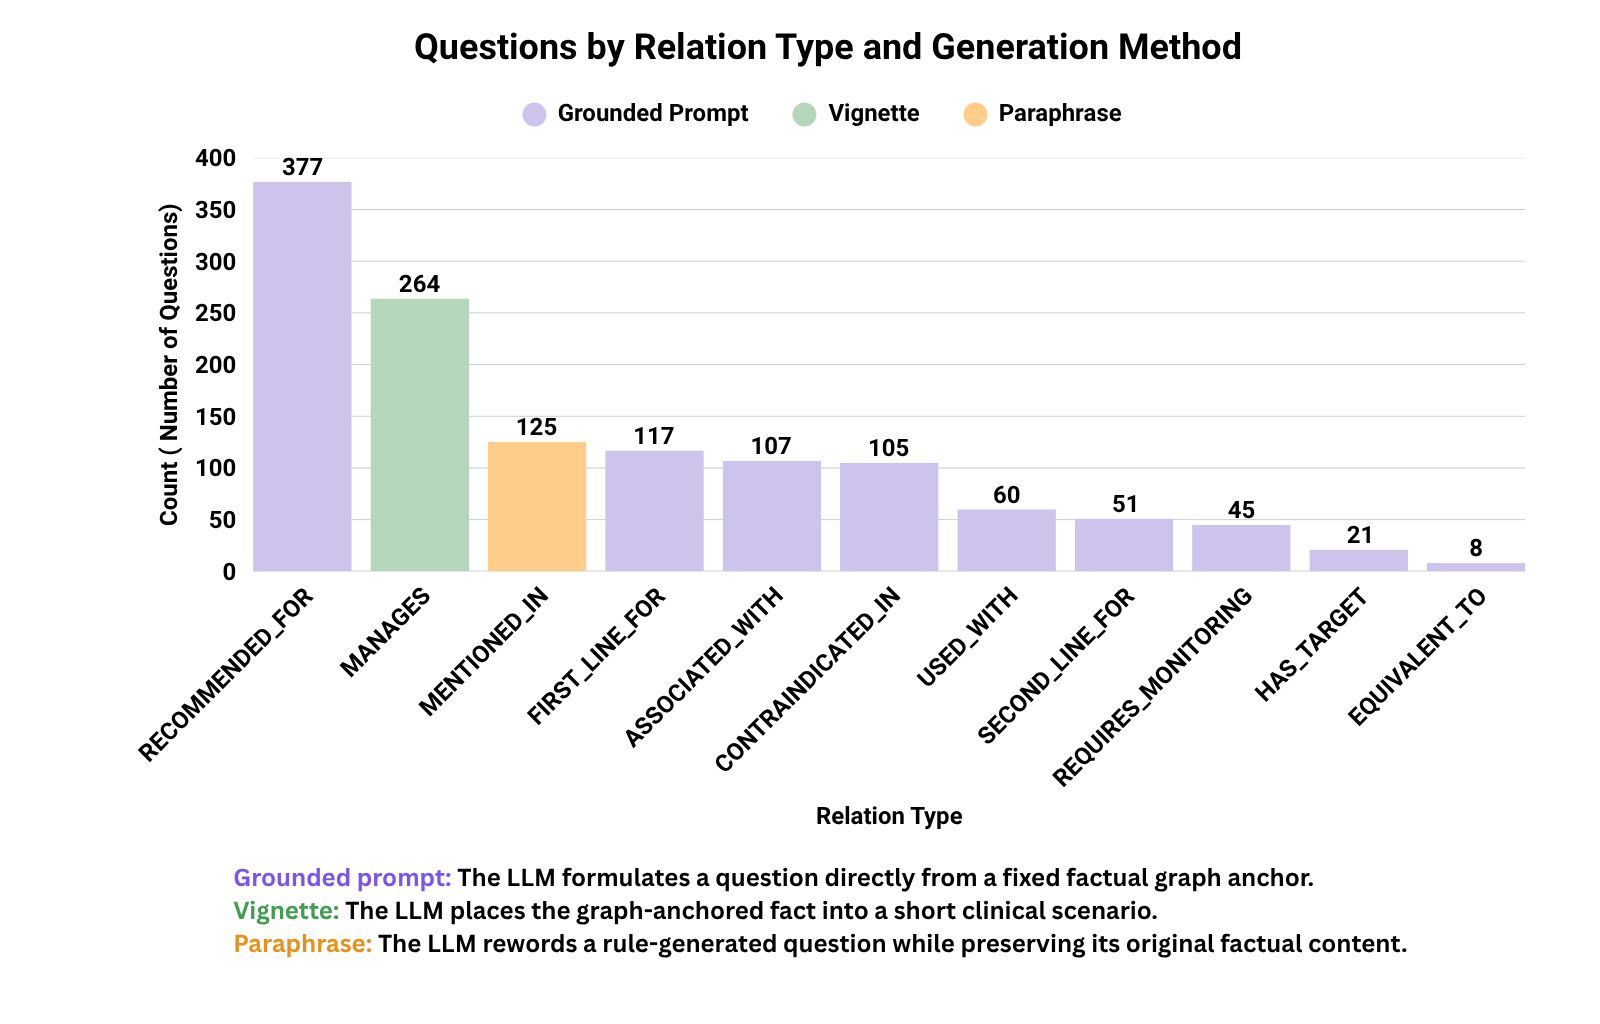
\includegraphics[width=\textwidth]{inc/figures/q_method.png}
    \caption{Question distribution by relation type and generation method.}
    \label{fig:q-method}
\end{figure}


Figure~\ref{fig:q-method} shows how the generated questions were distributed across the graph relation types and the three primary generation methods. The distribution reflects the fixed relation-to-method mapping used by the question-generation pipeline. Grounded prompts were used for relations where the answer could be directly formulated from the graph assertion, while clinical vignettes and template paraphrases were used for the corresponding relation types defined by the generation configuration.

\begin{figure}[!ht]
    \centering
    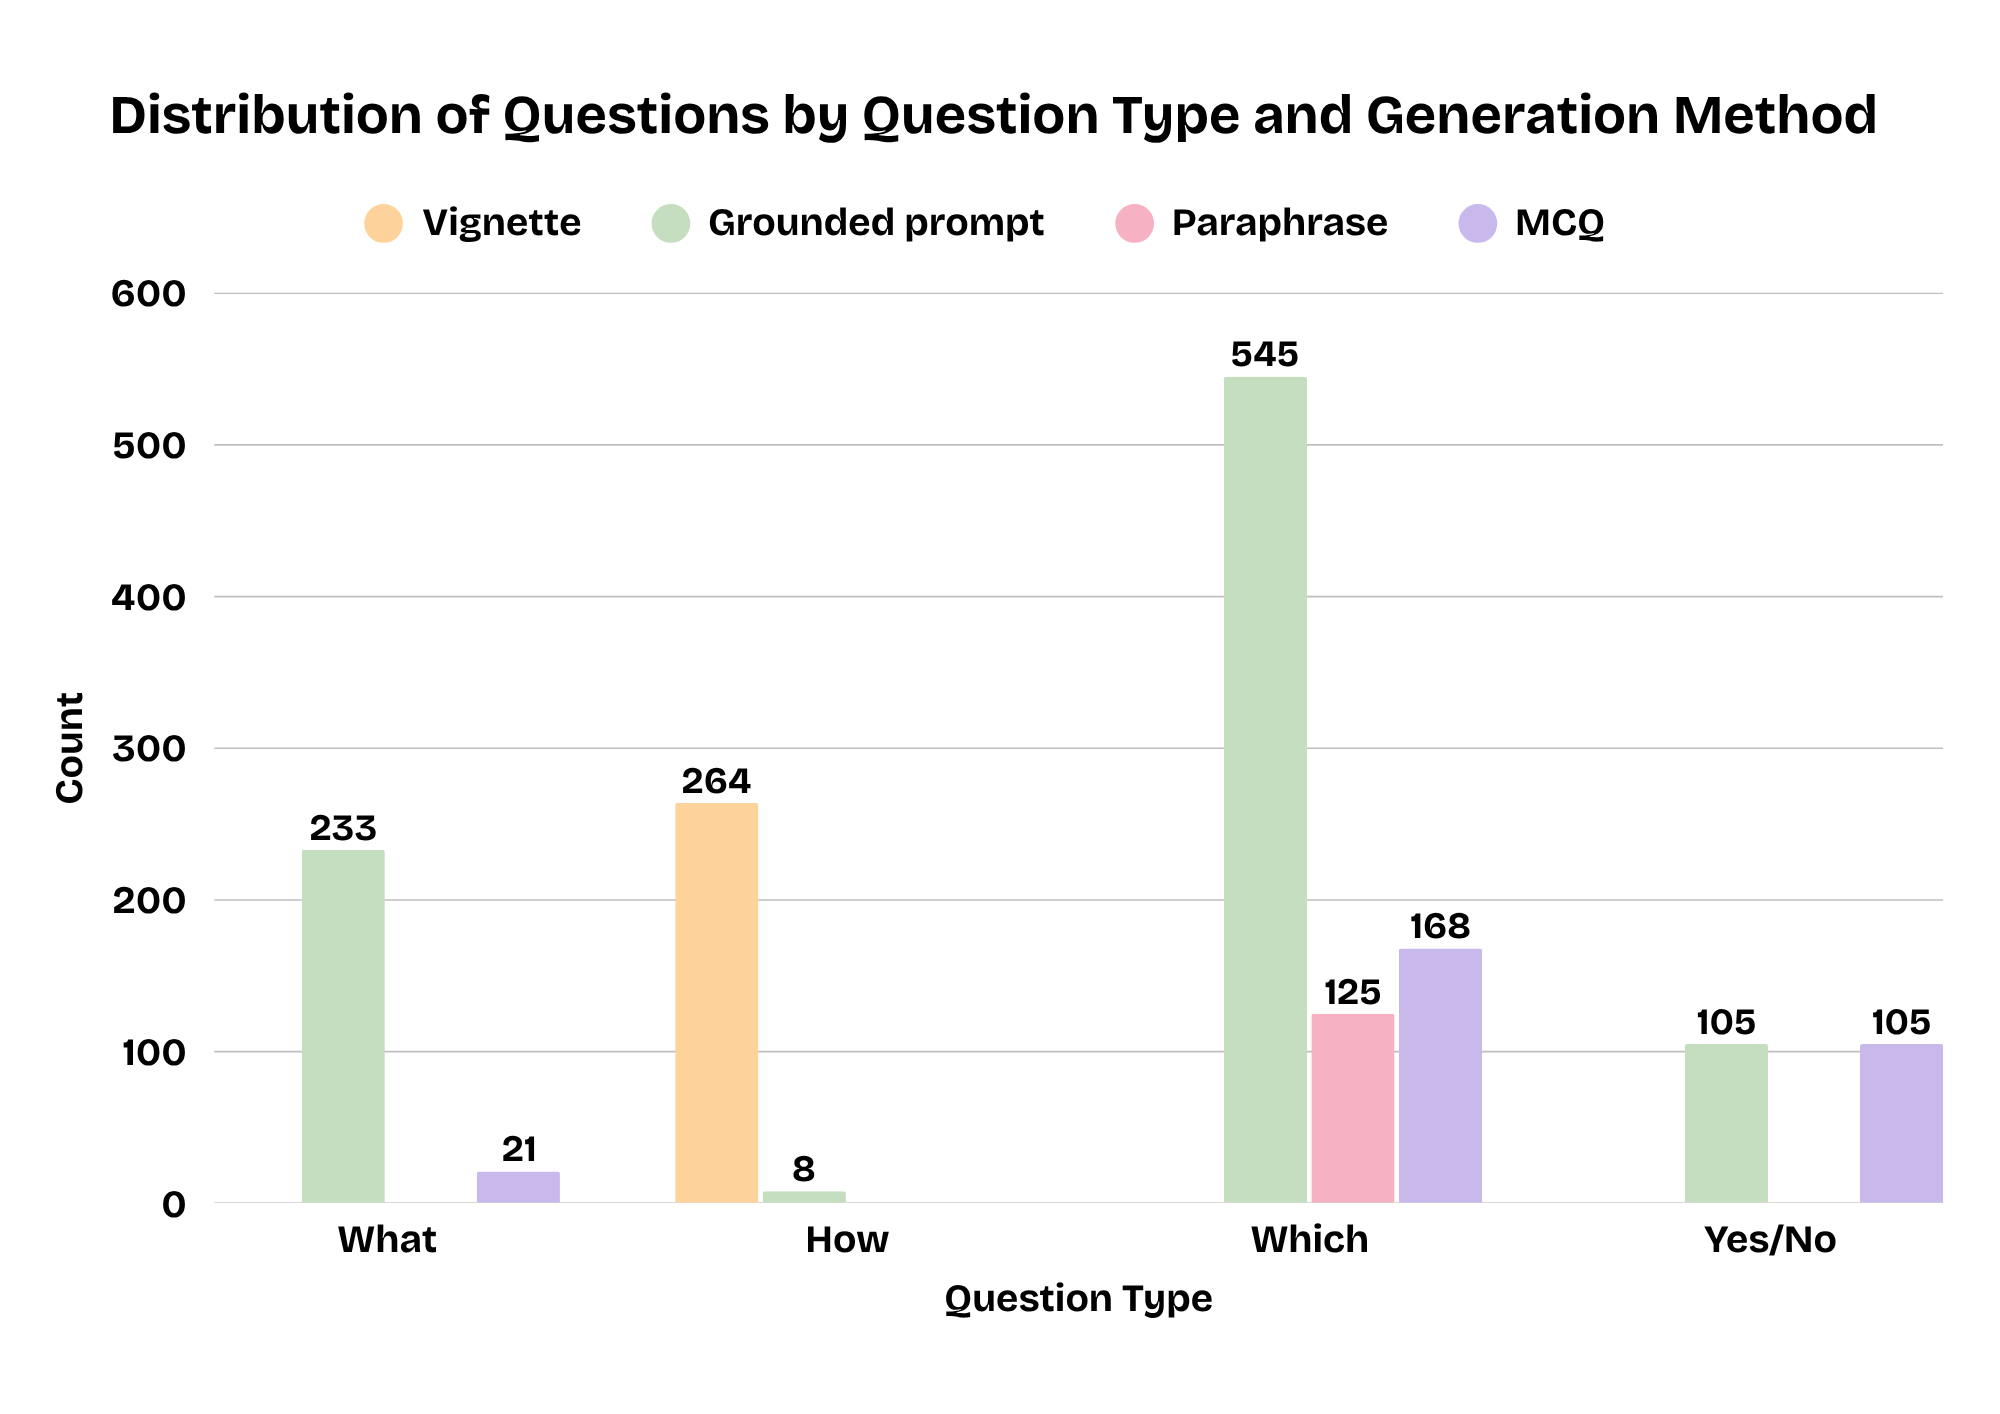
\includegraphics[width=\textwidth]{inc/figures/q_type.png}
    \caption{Distribution of accepted questions by question type, primary generation method, and MCQ format.}
    \label{fig:q-type}
\end{figure}

Figure~\ref{fig:q-type} shows the distribution of accepted questions across the four question types and the three primary generation methods. The figure also indicates which accepted questions were produced in multiple-choice format (MCQ). MCQ is treated as an output format rather than a separate generation method.

\subsection{Distribution by Generation Method and Question Type}
\label{sec:q-by-method}

\begin{table}[!ht]
\centering
\small
\begin{tabular}{lrr@{\hspace{1.5cm}}lrr}
\hline
\textbf{Method} & \textbf{N} & \textbf{\%} &
\textbf{Type} & \textbf{N} & \textbf{\%} \\
\hline
Graph-grounded prompt  & 899 & 69.7 & \textit{which}    & 676 & 52.4 \\
Clinical vignette      &    265  & 20.6 & \textit{how}  & 273 & 21.2 \\
Template paraphrase    &    125  & 9.7 & \textit{what}   & 233 & 18.1 \\
                       &         &      & \textit{yes/no} & 107 &  8.3 \\
\hline
\textbf{Total}         & 1{,}289 & 100  & \textbf{Total}  & 1{,}289 & 100 \\
\hline
\end{tabular}
\caption{Questions by generation method and question type in the full
         GPT-4o-mini catalogue.}
\label{tab:q-method}
\end{table}

The which form is the most frequent (52.4\%), driven primarily by \textsc{recommended\_for}, \textsc{first\_line\_for}, \textsc{second\_line\_for}, and the cross-guideline \textsc{mentioned\_in} questions. The how form accounts for 21.2\% and is dominated by the vignette-based \textsc{manages} relations. The yes/no form remains the least frequent (8.3\%) because it is restricted to \textsc{contraindicated\_in} edges.


\subsection{Cross-Guideline Questions}
\label{sec:cross-guideline-q}

The eight questions derived from \textsc{equivalent\_to} anchors are the only
ones in the catalogue requiring knowledge spanning two guidelines. Each anchor
pairs two \textsc{GlycaemicTarget} nodes from different organisations that
share the same normalised threshold. An example question from the
FPG $\geq 7.0$~mmol/L edge between ADA and Diabetes Canada:

\begin{quote}
\textit{What fasting plasma glucose threshold is shared by the ADA and
Diabetes Canada target nodes, and in what units does each guideline state
it?}
\end{quote}

This question type is not possible from a single-guideline pipeline in this corpus or by
extraction from raw text, because it depends on an \textsc{equivalent\_to}
edge that does not exist in any source document.

\subsection{Representative Examples}
\label{sec:q-examples}

Table~\ref{tab:q-examples} shows representative questions drawn from the
validated catalogue, grouped by generation method and question type. The
examples illustrate the linguistic variety the hybrid pipeline achieves
compared to a single fixed template: the grounded-prompt method produces
direct factual questions; the vignette method produces clinical scenario
questions that embed the same pharmacological fact in a patient narrative (the
patient details, such as age group, sex or symptoms, are added by the model
and are not drawn from the anchor);
and questions derived from \textsc{equivalent\_to} anchors require the
student to compare positions across two guidelines simultaneously.

\begin{table}[!ht]
\centering
\small\setlength{\tabcolsep}{6pt}
\begin{tabular}{p{2.4cm} p{2.8cm} p{8.0cm}}
\hline
\textbf{Method} & \textbf{Type} & \textbf{Question} \\
\hline
Graph-grounded prompt
  & \textit{which} (recall)
  & Which pharmacological approach is recommended for managing blood
    glucose in people with diabetes who are at higher risk of
    hypoglycaemia? \\[6pt]
Graph-grounded prompt
  & \textit{what} (recall)
  & What fasting plasma glucose level is used as the threshold for
    identifying individuals at risk of developing type~2 diabetes? \\[6pt]
Graph-grounded prompt + MCQ
  & \textit{what} (recall)
  & In a patient presenting with classic symptoms of hyperglycaemia,
    what random plasma glucose value meets the diagnostic threshold
    for diabetes mellitus?
    \newline
    \textit{A.}~$\geq 180.0$~mg/dL \quad
    \textit{B.}~$\geq 140.0$~mg/dL \quad
    \textit{C.}~$\geq 200.0$~mg/dL \quad
    \textit{D.}~$\geq 160.0$~mg/dL \\[6pt]
Clinical vignette
  & \textit{how} (application)
  & A middle-aged man with a history of type~2 diabetes and recently
    diagnosed stable heart failure presents for a routine medication
    review. He reports mild ankle swelling and reduced exercise
    tolerance. Which pharmacological management strategy should be
    prioritised given his dual diagnosis? \\[6pt]
Cross-guideline
  & \textit{how} (application)
  & How does the fasting plasma glucose threshold used to diagnose
    diabetes compare between the American Diabetes Association and
    Diabetes Canada guidelines? \\
\hline
\end{tabular}
\caption{Representative questions from the validated catalogue.}
\label{tab:q-examples}
\end{table}

\section{Evaluation of Question Quality}
\label{sec:exp_quality}

This section evaluates question quality beyond the automatic validator. A rule-based baseline is used to compare output variety, lexical diversity is assessed at catalogue level, and a sample from the partial Claude Opus 4.8 run is examined through independent clinical review.

\subsection{Baseline Definition}
\label{sec:exp_quality-baseline}

The baseline for comparison is a rule-only question generator that produces
one canonical question per anchor triple using a fixed directional template
per relation type. For a \textsc{recommended\_for} edge with source $v_s$ and
destination $v_d$, the canonical template produces: \textit{``Which drug is
recommended for $v_d$?''} with the answer fixed to $v_s$. No language model
is called, no reformulations are generated, and no MCQ distractors are
produced. Anchor consistency holds trivially here, because the question text
contains only the node names from the anchor. Hallucination in language
models is a well-documented problem~\cite{huang2025}; the validator is
designed specifically to catch faithfulness failures where the generated
text departs from the supplied anchor fact. The baseline represents the
minimum viable question catalogue: graph-anchored, consistently
structured, and producible without any LLM calls or additional cost.

The hybrid pipeline, described in Section~\ref{sec:exp_questions}, differs
from this baseline in three respects: the surface form of each question is
generated from an anchor-restricted prompt; reformulations
of the question are generated at up to three distinct phrasings; and
multiple-choice distractors are generated for selected relation types. The rule-only baseline is anchor-consistent by construction because its question and answer are assembled directly from the graph anchor. For the hybrid pipeline, anchor consistency is checked after language-model formulation by the rule-based validator, and only questions passing these checks enter the validated catalogue. Neither case implies that the underlying graph edge is clinically correct.

\subsection{Validator Analysis}
\label{sec:validator-analysis}

The validator applies three checks to every generated question. Check~1
verifies that the correct answer appears in the question text or is
recoverable as a named graph entity. Check~2 flags any number in the
generated question that was not present in the anchor's node properties
(with small integers 0--4 whitelisted as non-clinical). Check~3 verifies
that if a specific guideline is named in the question, it matches the anchor's
issuing organisation.

Nine questions were routed to \(\mathcal{Q}^-\), all because Check~2 detected numerical information in the generated question that was not represented among the numerical properties permitted by the validator. Six originated from \textsc{recommended\_for} relations, two from \textsc{contraindicated\_in}, and one from a \textsc{manages} relation. The flagged values included patient ages or age ranges, a postpartum duration, an eGFR range, and an age introduced in a vignette. Inspection showed that several of these values reflected information embedded in population or condition descriptions rather than newly invented clinical thresholds. The numerical validator is therefore deliberately conservative and can flag contextually appropriate numbers when they are not represented in the specific anchor properties it checks. The resulting 99.3\% acceptance rate measures consistency with the implemented validation rules rather than clinical accuracy.


\subsection{Automatic Metrics}
\label{sec:exp_quality-automatic}

Table~\ref{tab:quality-auto} compares the hybrid pipeline against the rule-only
baseline: the hybrid pipeline generates 294 multiple-choice questions and 3.38
phrasings per anchor on average, against none and exactly 1.00 for the rule-only
baseline. The validator pass rate is lower for the hybrid pipeline (99.3\%
against 100\%) for the reasons discussed in Section~\ref{sec:validator-analysis}.

\begin{table}[!ht]
\centering
\small\setlength{\tabcolsep}{8pt}
\begin{tabular}{lcc}
\hline
\textbf{Metric} & \textbf{Rule-only baseline} & \textbf{Hybrid pipeline} \\
\hline
Validator pass rate     & 100\%   & 99.3\% \\
Questions with MCQ      & 0       & 294 \\
Mean phrasings/anchor   & 1.00    & 3.38 \\
MSTTR (window 50)       & n/a     & 0.716 \\
Primary difficulty labels       & n/a       & 2 (recall, application)\\
\hline
\end{tabular}
\caption{Automatic metrics for the rule-only and hybrid pipelines.}
\label{tab:quality-auto}
\end{table}

The main quantitative difference between the two approaches is the variety of question forms produced.
The accepted GPT-4o-mini catalogue contains 1,280 primary questions and 3,048 stored reformulations, giving 4,328 phrasings in total. To describe this variation, the mean number of stored phrasings per accepted anchor is calculated as

\[
\text{Mean phrasings per anchor}
=
\frac{N_{\mathrm{primary}} + N_{\mathrm{reformulations}}}
     {N_{\mathrm{primary}}}.
\]

Since each primary question corresponds to one accepted graph anchor, this gives
\[
\frac{1280 + 3048}{1280} = 3.38
\]
stored phrasings per anchor.

Lexical diversity is measured using the Mean Segmental Type--Token Ratio (MSTTR)~\cite{Ahn2025}. Unlike the conventional type--token ratio, MSTTR reduces the effect of text length by calculating lexical diversity over equal-length, non-overlapping segments:

\[
\mathrm{MSTTR}
=
\frac{1}{k}\sum_{i=1}^{k}\frac{t_i}{w_i},
\]

where \(k\) is the number of segments, \(t_i\) is the number of unique word types in segment \(i\), and \(w_i\) is the number of tokens in that segment. Using a 50-token window across the primary questions and their reformulations gives an MSTTR of 0.716.

The accepted catalogue also contains 294 questions with MCQ options. Primary questions are labelled as either recall or application depending on the generation method, while the reformulations additionally include analysis variants. In comparison, the rule-only baseline produces a single phrasing per anchor, does not generate MCQ options, and does not assign difficulty labels.

\subsection{Human Clinical Review}
\label{sec:exp_quality-human}

A sample of 30 questions from the 491-question partial Claude Opus 4.8 catalogue was reviewed for clinical soundness by two medical doctors. The questions were presented without the graph anchors that produced
them, so that each reviewer judged the question on its own clinical merits
rather than against the system's intended answer. The two review sets of 15
questions each were non-overlapping and sampled across generation methods in
proportion to their frequency in the catalogue.

Evaluation of clinical NLP systems often relies on comparison against
expert-annotated reference standards \cite{uzuner2011}, and for
generated clinical text, evaluation by physicians has been used to assess
quality along clinical dimensions \cite{singhal2025}.
Each reviewer was asked to mark each question as clinically correct or
incorrect, and to provide one line of explanation for any question marked
incorrect. Both reviewers are qualified medical doctors from India and were contacted through the author's personal network. Dr. Mounika is currently in the final year of postgraduate training in Obstetrics and Gynaecology. Dr. Aakanksha completed her undergraduate medical education in India, and is currently preparing for the Fachsprachprüfung (FSP) in Heidelberg, Germany as part of the process of continuing medical practice in Germany. Both participated voluntarily and without compensation, and agreed to take part and to be described in this thesis. The review involved no patients and no personal data beyond the reviewers' professional background reported here. Each reviewed a separate set of 15 questions, so the
two sets do not overlap and no question was seen by both reviewers. Reviewers
worked independently and were not in contact with each other during the
review. They were shown the question text only, without the graph anchor, the
answer key, or the source guideline passage, so each judgement was made on the
question as a learner would encounter it. The reviewers were also not informed which language model had generated the questions. Because the guidelines in the corpus are American, British, Canadian, and international, reviewers were asked to indicate where a flag reflected a difference from routine practice in their own clinical context rather than a factual error in the question.

The human review showed that most questions were considered acceptable, while several issues were identified in the reviewed sample. Table~\ref{tab:quality-human} summarises the individual review results, while Figure~\ref{fig:review} shows the distribution of the review outcomes for the two reviewers. The following discussion examines the identified issues in more detail.

\begin{table}[!ht]
\centering
\small\setlength{\tabcolsep}{5pt}
\begin{tabular}{p{0.5cm} p{1.8cm} p{5.0cm} p{4.8cm}}
\hline
\textbf{Q} & \textbf{Reviewer} & \textbf{Reviewer comment} & \textbf{Root cause} \\
\hline
Q9
  & Dr. Aakanksha
  & Metformin identified as managing hypoglycaemic events; sulfonylureas
    are the drug class associated with hypoglycaemia
  & Extraction error: the source passage does not support the extracted \texttt{metformin --MANAGES--> hypoglycaemic events} relation \\[4pt]

Q15
  & Dr. Aakanksha
  & NHS Path to Remission recommended for Heart Failure; SGLT2 inhibitors
    are the standard pharmacological approach for T2DM with Heart Failure
    & Extraction error: the source passage does not support the extracted
    \texttt{manages} relation between this programme and Heart Failure \\[4pt]
Q3
  & Dr. Mounika
  & No specific antidiabetic is recommended for fractures; perioperative
    glycaemic control is managed by insulin dose adjustment only
  & Extraction error: the source passage does not support the extracted \texttt{insulin --RECOMMENDED\_FOR--> fractures} relation \\[4pt]
Q6
  & Dr. Mounika
  & Bariatric surgery for T2DM is evidence-based but not routine practice;
    noted as practised differently in India
  & Clinical scope: ADA and IDF guidelines do recommend metabolic surgery
    for eligible adults with T2DM; not an extraction error \\
\hline
\end{tabular}
\caption{Human clinical review results.}
\label{tab:quality-human}
\end{table}

\begin{figure}[!ht]
    \centering
    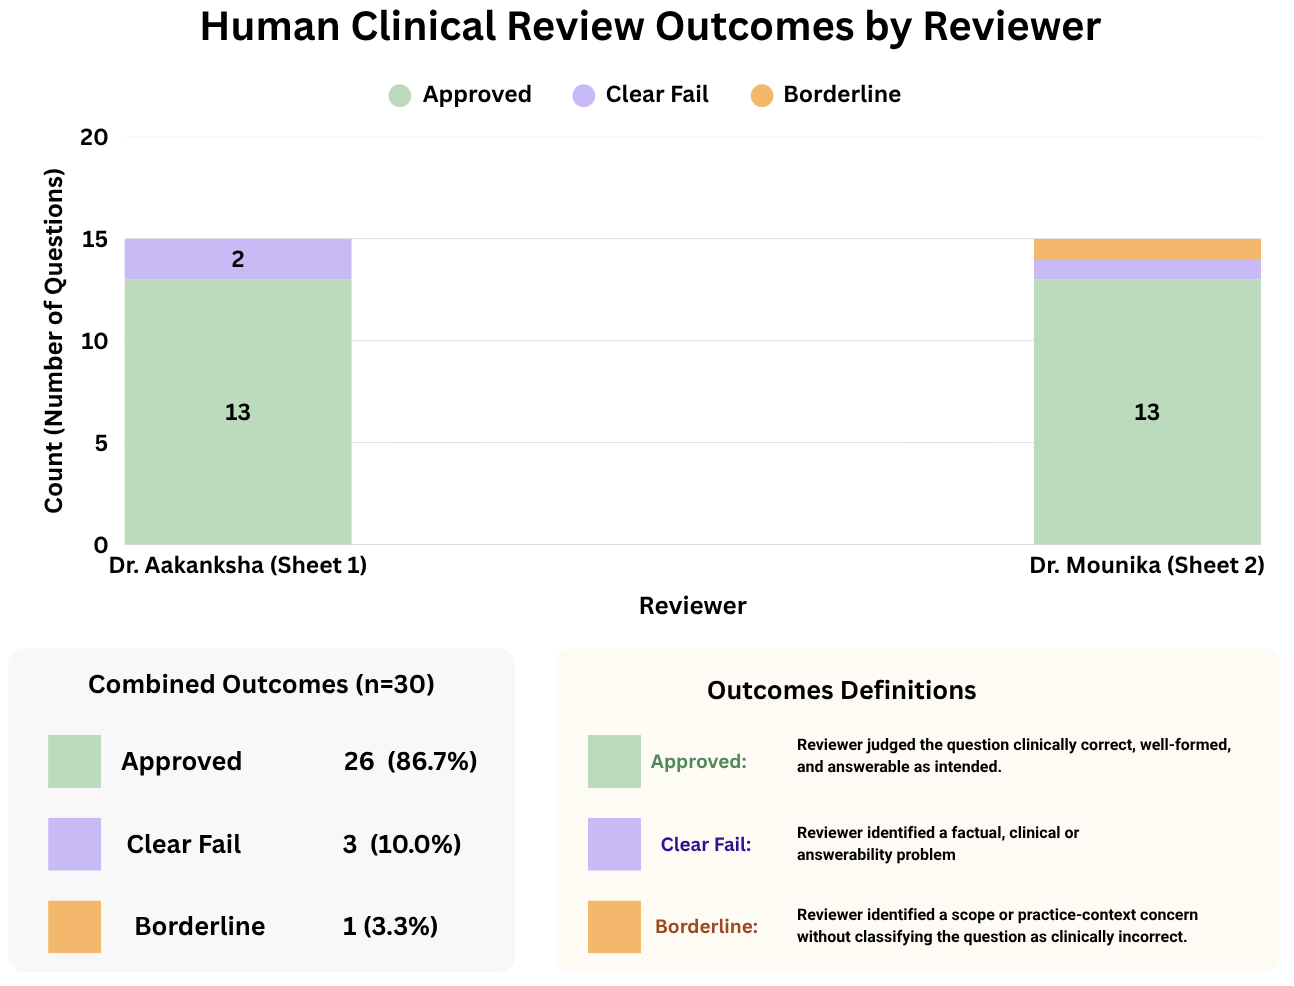
\includegraphics[width=0.75\textwidth]{inc/figures/review.png}
    \caption{Human clinical review outcomes by reviewer.}
    \label{fig:review}
\end{figure}


Of the 30 reviewed questions, 26 were accepted without qualification.
Three were classified as clear failures and were traced to incorrect
relations in the Knowledge Graph. One additional question (Q6) was
flagged because its content, although supported by the source guidelines,
was outside routine practice in the reviewer's clinical context. This
case is therefore treated as a clinical-scope flag rather than a factual
error.

Within this sample, all three clear failures originated from incorrect
graph relations rather than from the question-formulation step. The
sample is too small to establish a general reliability rate, but it
indicates that graph quality was the main source of factual error among
the reviewed questions.

One additional question was flagged by Dr. Aakanksha (Q5), which asked how the ADA
and IDF diagnostic thresholds for the 2-hour oral glucose tolerance test
compare. The reviewer noted that both guidelines use the same
threshold of $\geq 11.1$~mmol/L, which is the intended answer to the
question. This confirms that the cross-guideline comparison question type
produced from \textsc{equivalent\_to} edges is answerable. It is not counted as a failure.



\subsection{Comparison with Baseline}
\label{sec:exp_quality-comparison}

Clinical correctness against the original guideline sources was not independently measured for the rule-only baseline, so the comparison is limited to properties of the generated catalogue rather than clinical accuracy.The accepted hybrid catalogue contains 1,280 primary questions together with 3,048 additional reformulations and 294 questions with MCQ options. Primary questions carry recall or application difficulty labels, while the stored reformulations additionally include recall, application, and analysis variants. This provides a wider range of question forms than the fixed single-phrasing rule-only baseline. Whether this additional variety translates into improved learning outcomes is not evaluated in this thesis and remains a question for future study.



\section{Limitations}
\label{sec:exp_limitations}

The experiments and the final implementation showed several limitations
that would need to be addressed in further work.

\paragraph{Entity matching.}
Drug and clinical-condition names are merged using fixed alias lists.
This works for the variants included in those lists, but an alternative
name that is not listed can remain as a separate node. The current
implementation therefore depends on knowing common naming variations in
advance. Extending the alias lists would improve coverage, although the
additional mappings would need to be checked to avoid merging different
clinical concepts.

\paragraph{Cross-guideline target comparison.}
The current \textsc{equivalent\_to} comparison is limited to
plasma-glucose targets that have a value in mmol/L. HbA1c targets are
also extracted, and conversions between percentage and mmol/mol are
stored, but these values are not included in the equivalence comparison.
The eight equivalence relations reported in this chapter therefore cover
only the plasma-glucose targets matched by the implemented criterion.

\paragraph{Condition scoping.}
The diabetes type of a numerical target is determined from the text in
which the target is extracted. If that text mentions both Type~1 and
Type~2 diabetes, or does not identify either one, the target is kept but
no disease-specific \textsc{has\_target} relation is added. This is safer
than assigning a default condition, but some targets consequently remain
without a Type~1 or Type~2 link. Section or document context could be used
in addition to the local text in a future version.

\paragraph{Contextual extraction.}

Contextual entity and relation extraction contributes directly to the final Knowledge Graph used by both question-generation runs. Although the LLM extractor is constrained through the prompt to predefined entity and relation types and is instructed not to introduce relations unsupported by the source passage, these constraints are not enforced independently against the original guideline after extraction. Errors introduced during contextual extraction can propagate into the final graph and subsequently into generated questions. This was observed during human review, where some clinically questionable questions remained consistent with incorrect or questionable graph relations. Since the question validator checks graph-anchor consistency rather than independently verifying the source guideline, such upstream errors are outside its scope. A systematic source-level evaluation of contextual extraction was not carried out and remains future work.

\paragraph{Generalisability.}
The pipeline was evaluated only on the diabetes guideline corpus used in
this thesis. Several ingestion rules are specific to the four publishing
formats in the corpus. For example, the implementation contains separate
handling for ADA recommendation blocks, NICE document structure, IDF
care-level recommendations, and Diabetes Canada text extraction. A new
guideline family may therefore require additional document-specific
handling before the rest of the pipeline can be applied.